\chapter{Reazioni in fase condensata}
Le sostanze reagenti non si trovano sempre come le uniche specie presenti e, soprattutto nelle reazioni tra fasi condensate, � spesso presente una sostanza (\textsl{solvente}) che interagisce con esse. 

Gli effetti del solvente possono essere raggruppati in:
\begin{itemize}
	\item \textsl{Effetto cella}: il solvente si dispone in maniera ordinata intorno ai reagenti.
	\item \textsl{Effetto ionizzante}: si formano i cationi perch� stabilizzati dalla cella di solvente.
	\item \textsl{Solvatazione}: effetti di interazione tra solvente e soluto.
\end{itemize}
Consideriamo la generica reazione:
\begin{equation}
	X^- + CH_3Y \rightarrow XCH_3 + Y^-
	\label{eq:sol:RxnGenerica}
\end{equation}
possiamo diagrammare l'andamento secondo le coordinate di reazione (Figura \ref{fig:ELambda_Rxn_XCH3Y}),
\begin{figure}[htbp]
	\centering
		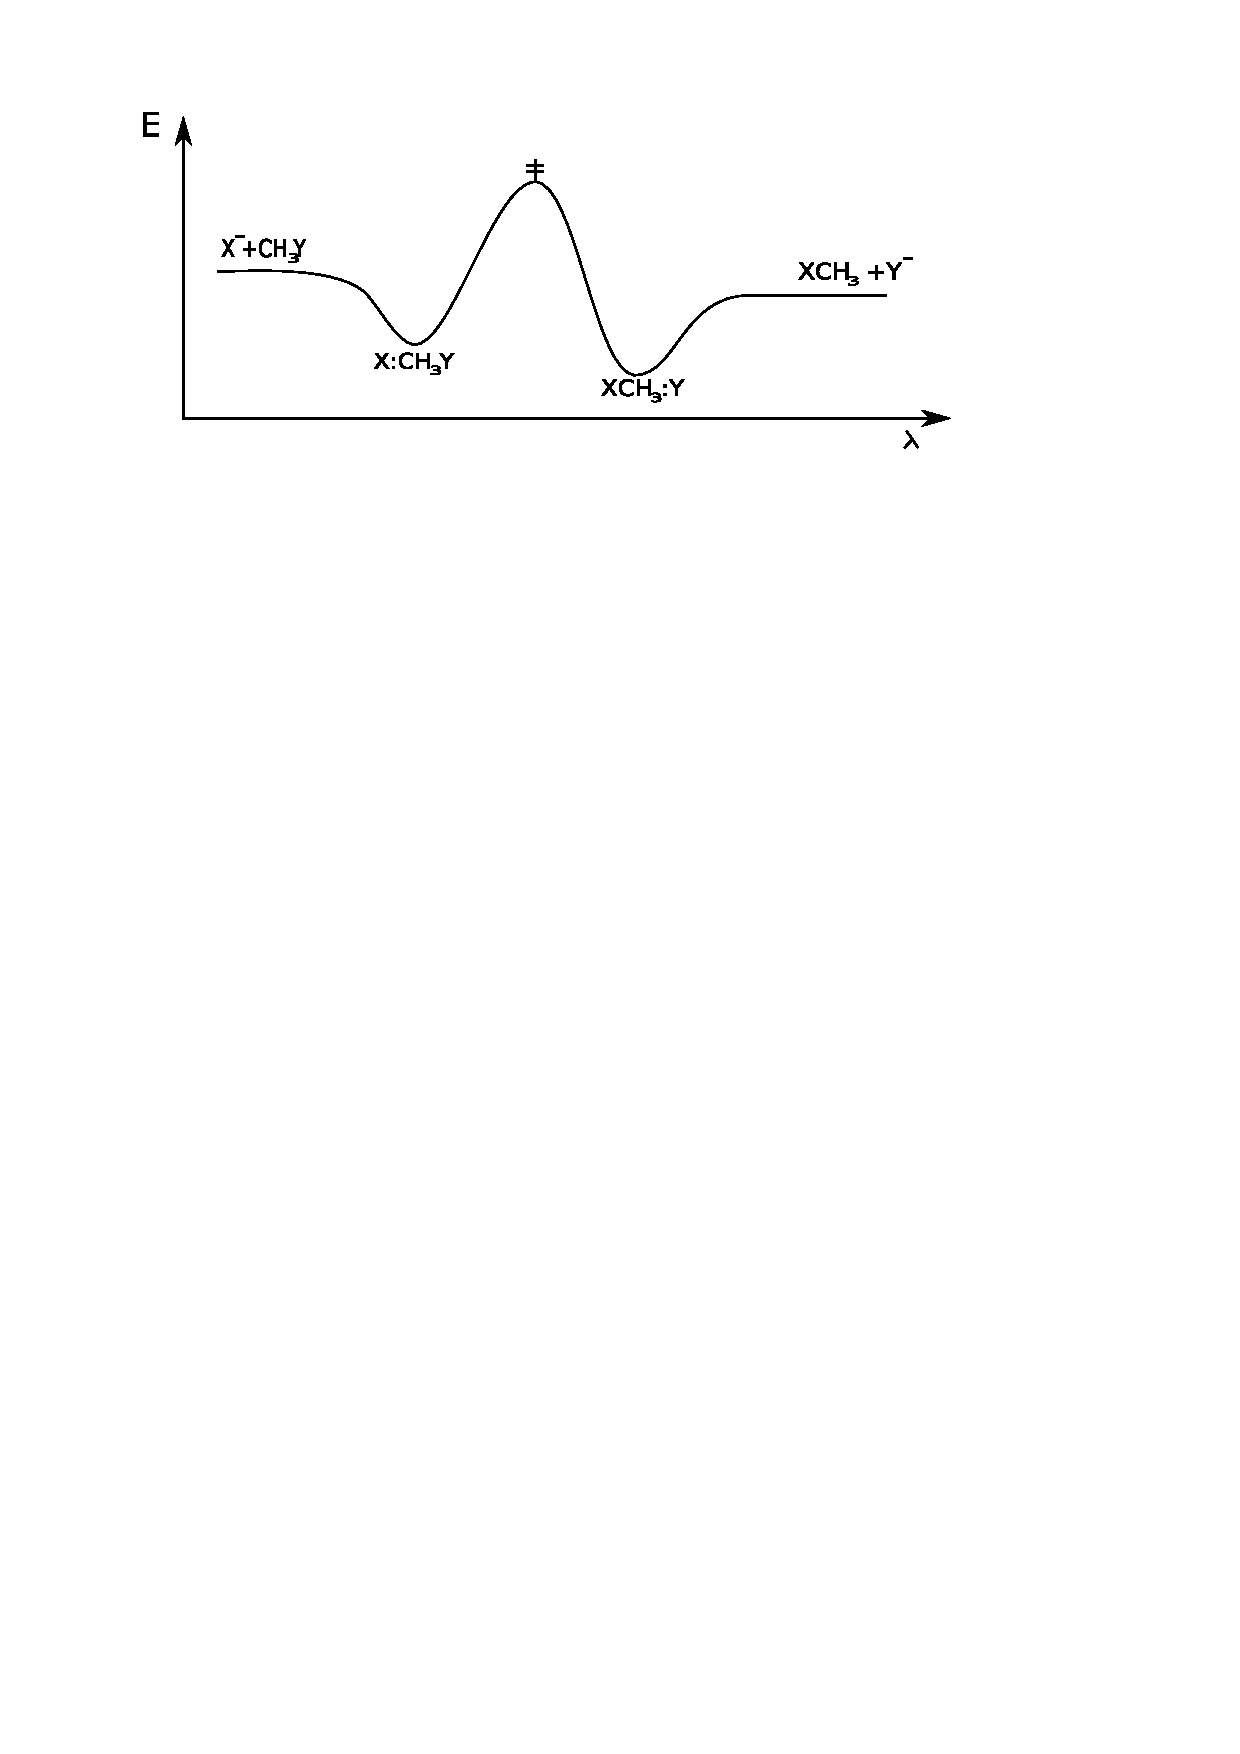
\includegraphics[height=4cm]{image/ELambdaXCH3Y.pdf}
	\caption{\small Andamento dell'energia (E) rispetto alla coordinata di reazione ($\lambda$).}
	\label{fig:ELambda_Rxn_XCH3Y}
\end{figure}
nel quale si nota la formazione dei complessi $X:CH_3Y$ e $Y:CH_3X$.\\
Se la stessa reazione avvenisse in presenza di un solvente noteremmo l'andamento risontrato in Figura \ref{fig:ELambda_Rxn_XCH3Y_Solvente},
\begin{figure}[htbp]
	\centering
		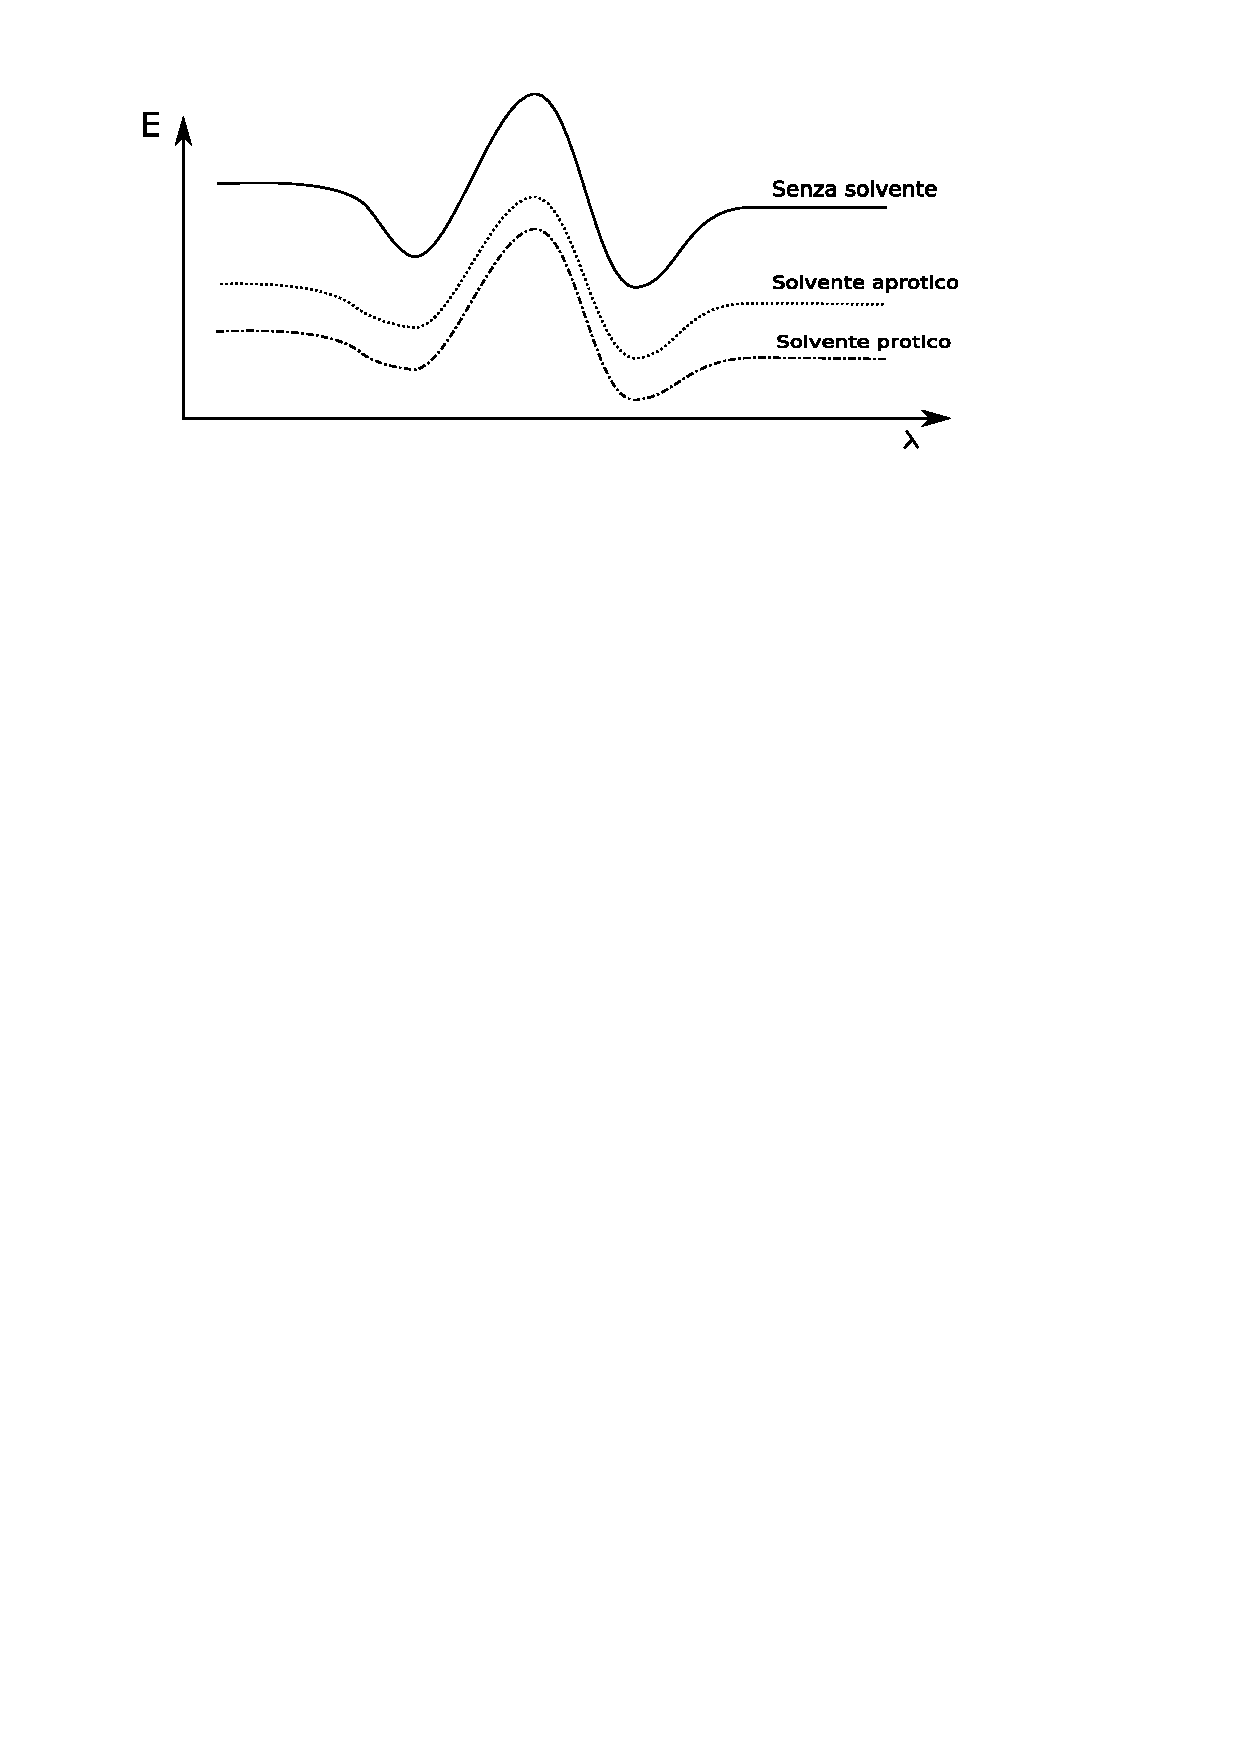
\includegraphics[height=4cm]{image/ELambdaXCH3YSolvente.pdf}
	\caption{\small Andamento dell'energia (E) rispetto alla coordinata di reazione ($\lambda$) per la reazione in soluzione.}
	\label{fig:ELambda_Rxn_XCH3Y_Solvente}
\end{figure}
dove la differenza energetica tra le specie reagenti e quelle in soluzione � definita come $\Delta H$ di solvatazione. Nell'intorno del complesso attivato si ha una diminuzione del $\Delta H_{solv}$ essendo la carica pi� delocalizzata, da cui l'effetto del solvente perde parte della sua importanza, quindi � anche vero che l'energia di attivazione per le reazioni in soluzione � maggiore che non per le specie pure.

Altro fattore importante all'interno delle reazioni in soluzione � il tipo di controllo che la reazione subsce, infatti:
\begin{equation}
	A + B \rightleftharpoons AB \rightleftharpoons AB^{\ddagger} \rightarrow C
	\label{eq:sol:RxnGenerica2}
\end{equation}

Il controllo � di tipo \textsl{cinetico} se la velocit� di formazione del complesso attivato $AB^{\ddagger}$ a determinare la velocit� di reazione.

Il controllo � di tipo \textsl{diffusivo} se la velocit� di formazione del complesso $AB$ a determinare la velocit� di reazione.

Consideriamo il caso di trovarci sotto controllo diffusivo abbiamo:
\begin{equation}
	R = \frac{k_B \cdot T}{h} \cdot [AB^{\ddagger}]
	\label{eq:sol:VelocitaReazione}
\end{equation}
essendo immediata la formazione del complesso attivato la sua reazione sar� all'equilibrio, quindi:
\begin{equation}
	K_{eq}^{\ddagger} = \frac{[AB^{\ddagger}]}{[A] \cdot [B]} = \frac{a_{AB^{\ddagger}}}{a_A \cdot a_B}
	\label{eq:sol:KeqIntermedio}
\end{equation}
essendo anche $a_i = {C_i} \cdot \gamma_i$ ricaviamo:
\begin{equation}
	K_{eq}^{\ddagger} = \frac{C_{AB^{\ddagger}}}{C_A \cdot C_B} \cdot
											\frac{\gamma_{AB^{\ddagger}}}{\gamma_A \cdot \gamma_B}
	\label{eq:sol:KeqIntermedioGamma}
\end{equation}
da cui si ricava:
\begin{equation}
	R = \frac{k_B \cdot T}{h} \cdot K_{eq}^{\ddagger} \cdot
			\frac{\gamma_{AB^{\ddagger}}}{\gamma_A \cdot \gamma_B} \cdot
			C_A \cdot C_B
	\label{eq:sol:ConcIntermedio}
\end{equation}
Essendo anche:
\begin{equation}
	\frac{k_B \cdot T}{h} \cdot K_{eq}^{\ddagger} = cost = K_{(T)}^0
	\label{eq:sol:K0T}
\end{equation}
e riunendo
\begin{equation}
	 K_{(T)} = K_{(T)}^0 \cdot \frac{\gamma_{AB^{\ddagger}}}{\gamma_A \cdot \gamma_B}
	\label{eq:sol:KT}
\end{equation}
otterremmo:
\begin{equation}
	R = K_{(T)} \cdot C_A \cdot C_B
	\label{eq:sol:VelReazioneKo}
\end{equation}

\section{Teoria di Br�nsted-Bjerron}
La determinazione del coefficiente di attivit� delle specie in soluzione pu� essere ottenuta dalle teoria di Br�nsted\footnote{Br�nsted, Johannes, chimico danese.}-Bjerron\footnote{Chi era...} che deriva della teoria di Debye\footnote{Debye, Peter Joseph Wilhelm (Maastricht 1884 - Ithaca, New York 1966), fisico-chimico statunitense di origine olandese.}-H\"uckel\footnote{H\"uckel, Erich assistente di Debye.}.

Queste teorie sono valide per le specie ioniche (in cui � importante l'effetto solvente) e i coefficienti di attivit� si possono ottenere da:
\begin{equation}
	\ln \gamma_i = -0,509 \cdot z_i^2 \cdot \sqrt{I}
	\label{eq:sol:lnGamma}
\end{equation}
dove indichiamo con:
\begin{equation}
	I = \frac{1}{2} \cdot \sum_j m_j z_j^2
	\label{eq:sol:IDebyeHuchel}
\end{equation}
dove $m_j$ indica la molalit� della specie $j$-esima in soluzione e $z_j$ la carica dello ione.

Per quanto visto prima (equazione \ref{eq:sol:KT}), logaritmando, abbiamo:
\begin{equation}
	\log K_{(T)} = \log K_{(T)}^0 + \log \gamma_{AB^{\ddagger}} - \log \gamma_A  - \log \gamma_B
	\label{eq:sol:logKT}
\end{equation}
e per la teoria di Debye-H\"uckel otteniamo:
\begin{equation}
	\frac{\log K_{(T)}}{\log K_{(T)}^0} = - 0,509 \cdot z_{AB^{\ddagger}}^2 \cdot \sqrt{I} +
																					0,509 \cdot z_A^2 \cdot \sqrt{I} +
																					0,509 \cdot z_B^2 \cdot \sqrt{I}
	\label{eq:sol:logKT}
\end{equation}
Per la legge della conservazione delle cariche $z_{AB^{\ddagger}} = z_A + z_B$ e quindi:
\begin{equation}
	\frac{\log K_{(T)}}{\log K_{(T)}^0} = - 0,509 \cdot \sqrt{I} \cdot 
								\left[ z_A^2 + z_B^2 - (z_A + z_B)^2 \right] = 
								-1,018 \cdot \sqrt{I} \cdot z_A \cdot z_B
	\label{eq:sol:logKTFinale}
\end{equation}
